\documentclass[tikz,border=5mm]{standalone}
\begin{document}
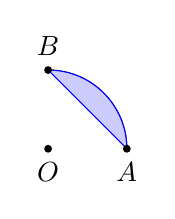
\begin{tikzpicture}
    % 绘制圆弧
    \draw (1,0) arc (0:90:1cm);
    
    % 填充圆弧
    \filldraw[fill=blue!20!white, draw=blue] (1,0) arc (0:90:1cm) -- cycle;
    
    % 标注圆心
    \node [circle,fill=black,inner sep=1pt,label=below:$O$] at (0,0) {};
    
    % 标注弧端点
    \node [circle,fill=black,inner sep=1pt,label=below:$A$] at (1,0) {};
    \node [circle,fill=black,inner sep=1pt,label=above:$B$] at (0,1) {};
    
\end{tikzpicture}
\end{document}